\documentclass[a4paper, 11pt]{report}

\usepackage[utf8]{inputenc}                                                      
\usepackage[french]{babel}                                                       
\usepackage[T1]{fontenc}  
\usepackage[utf8]{inputenc}                                                      
\usepackage[french]{babel}                                                       
\usepackage[T1]{fontenc}                                                         
\usepackage[pdftex]{graphicx}                                                    
\usepackage{url}                                                                 
\usepackage{longtable}
\usepackage[bookmarks, colorlinks=false, pdfborder={0 0 0},
	pdftitle={Medicagenda}, 
	pdfauthor={Knop Florian, Kriwin Paul, Placentino Simon},
	pdfsubject={Medicagenda},           
pdfkeywords={UML, ISO/IEC 14882:2011, Medicagenda, Projet, analyse, ESI}]{hyperref}   

\newcommand{\HRule}{\rule{\linewidth}{0.5mm}}    

\begin{document}
\begin{titlepage}
	\begin{center}

		
\includegraphics[keepaspectratio=true,width=0.20\textwidth]{../ressources/logo}\\[1cm]

		\textsc{\LARGE H.E.B. Ecole Superieur d'Informatique}\\[1.5cm]

		\textsc{\Large Laboratoire d'analyse : Projet d'analyse}\\[0.5cm]
		\textsc{\Large Modèle Conceptuel des Données}\\[0.5cm]

		\HRule \\[0.4cm]
		{\huge \bfseries Medicagenda \\[0.4cm]}
		\HRule \\[1.5cm]

		\noindent
		\begin{minipage}[t]{0.4\textwidth}
			\begin{flushleft} \large
				\emph{Auteurs:}\\
				Florian \textsc{Knop} \href{mailto:39310@heb.be}{39310@heb.be}\\
				Paul \textsc{Kriwin} \href{mailto:39171@heb.be}{39171@heb.be}\\
				Simon \textsc{Placentino} \href{mailto:39631@heb.be}{39631@heb.be}\
			\end{flushleft}
		\end{minipage}%
		\begin{minipage}[t]{0.4\textwidth}
			\begin{flushright} \large
				\emph{Titulaire du cours:} \\
				Mr.~Nicolas \textsc{Pettiaux}
				\href{mailto:npettiaux@heb.be}{npettiaux@heb.be}
			\end{flushright}
		\end{minipage}

		\vfill

		{\large \today}

	\end{center}
	\clearpage\null\newpage
\end{titlepage}

\tableofcontents

\chapter{Modèle conceptuel des données}

\section{Introduction}

\subsection{Objectifs du document}

Cette section sert à documenter et valider les éléments persistants qui devront
être stockés dans le système informatique de la gestion de calendriers de mèdecins.

\subsection{Domaine de définition du document}

Cette section reprend la description du diagramme métier (diagramme de classes) de la gestion de 
calendriers de mèdecins.

\subsection{Définitions, acronymes et abréviations}

\begin{enumerate}

\item \texttt{INAMI} : Institut national d'assurance maladie invalidité.

\end{enumerate}

\subsection{Références}

Enoncé du travail de synthèse sur la gestion de calendriers de mèdecins.

\newpage
\section{Diagramme(s) de classe(s)}

\begin{figure}[hb]
    \centering
    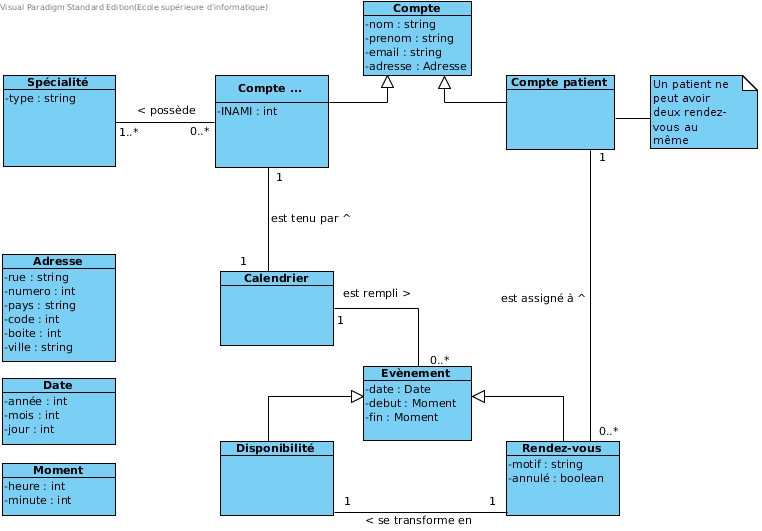
\includegraphics[scale=0.4]{MCD.jpg}
    \caption{Diagramme de classes Medicagenda}
\end{figure}

\newpage
\section{Classe(s)}


\subsection{Adresse}

\subsubsection{Définition}

Une adresse représente l'adresse postale d'une personne physique.

\subsubsection{Identifiant}

Tous les attributs d'une adresse forment un identifiant.

\subsubsection{Attributs}

\begin{itemize}
    \item rue
    \item numero
    \item ville
    \item pays
    \item code (= code postal)
    \item boite (optionnel)
\end{itemize}

\subsubsection{Contraintes d'intégrité}

Aucune.

\subsection{Calendrier}

\subsubsection{Définition}

Le calendrier représente tous les évènements futurs et permet
au mèdecin d'organiser ces évènements. \\
Un client peut ajouter un rendez-vous au calendrier d'un mèdecin.

\subsubsection{Identifiant}

Mèdecin.INAMI

\subsubsection{Attributs}

Aucun.

\subsubsection{Contraintes d'intégrité}

Aucune.

\subsubsection{Condition de création / suppression d'un objet ou de la classe}

A la création d'un compte mèdecin, un calendrier est créé pour ce mèdecin. 
Il n'est pas supprimé.


\subsection{Compte}

\subsubsection{Définition}

Un compte représente un compte sur le site en ligne. Un compte permet la gestion 
d'un calendrier ainsi que des paramètres personnels du client. \\
\texttt{Compte} est la super-classe de \texttt{Compte client} et \texttt{Compte Mèdecin}. 

\subsubsection{Identifiant}

Compte.e-mail

\subsubsection{Attributs}

\begin{itemize}
    \item Nom
    \item Prénom
    \item E-mail
    \item Adresse
\end{itemize}

\subsubsection{Contraintes d'intégrité}

Aucune.

\subsubsection{Condition de création / suppression d'un objet ou de la classe}

Un compte est créé par un mèdecin pour un client, ou par un mèdecin pour lui-même
ou par un client pour lui-même.
Une fois créé, il n'y a pas de possibilité de supression.


\subsection{Compte mèdecin}

\subsubsection{Définition}

Un compte mèdecin est un type de compte permettant au mèdecin de gérer ses rendez-vous et disponibilités
gràce au \texttt{calendrier}.

\subsubsection{Identifiant}

Identifiant de \texttt{Compte}.

\subsubsection{Attributs}

Attributs de \texttt{Compte}.

\subsubsection{Contraintes d'intégrité}

Aucune.

\subsubsection{Condition de création / suppression d'un objet ou de la classe}

Voir \texttt{Compte}.

\subsection{Compte patient}

\subsubsection{Définition}

Un compte client est un type de compte permettant au client d'ajouter des rendez-vous avec un mèdecin.
Un client peut modifier ses paramètres dans son espace client.

\subsubsection{Identifiant}

Identifiant de \texttt{Compte}.

\subsubsection{Attributs}

Attributs de \texttt{Compte}.

\subsubsection{Contraintes d'intégrité}

Aucune.

\subsubsection{Condition de création / suppression d'un objet ou de la classe}

Voir \texttt{Compte}.

\subsection{Date}

\subsubsection{Définition}

Une date représente une date représentée par un jour, un mois et une année.

\subsubsection{Identifiant}

Date.jour + Date.mois + Date.année

\subsubsection{Attributs}

\begin{itemize}

    \item{jour}
    \item{mois}
    \item{année}

\end{itemize}

\subsubsection{Contraintes d'intégrité}

\begin{itemize}
    \item Un jour prend les valeurs entre 1 et 31.
    \item Un mois prend les valeurs entre 1 et 12.
    \item La valeur maximale du jour dépend du mois (30 / 31 / 28 / 28).
\end{itemize}

\subsubsection{Condition de création / suppression d'un objet ou de la classe}

\subsection{Disponibilité}

\subsubsection{Définition}

Une disponibilité est une plage horaire dans laquelle un mèdecin accepte
des nouveaux rendez-vous.

\subsubsection{Identifiant}

Événement.date + Événement.debut + Événement.fin

\subsubsection{Attributs}

Voir \texttt{Événement}.

\subsubsection{Contraintes d'intégrité}

Voir \texttt{Événement}.

\subsubsection{Condition de création / suppression d'un objet ou de la classe}

Une disponibilité est créé lorsqu'un mèdecin décide d'accepter de nouveaux rendez-vous ou quand un
rendez-vous a été annulé par un client. Dans ce cas, le rendez-vous est transformé en disponibilité.

\subsection{Événement}

\subsubsection{Définition}

Un évènement est un horaire pendant lequel le mèdecin peut recevoir un patient ou en accepter de nouveaux.

\subsubsection{Identifiant}

Événement.date + Événement.debut + Événement.fin

\subsubsection{Attributs}

\begin{itemize}
    \item date
    \item début
    \item fin
\end{itemize}

\texttt{début} et \texttt{fin} représentent des heures/minutes de début et fin d'un évènement.

\subsubsection{Contraintes d'intégrité}

fin > début.

\subsubsection{Condition de création / suppression d'un objet ou de la classe}

Un évènement est soit créé par un mèdecin, soit par un client. Une fois l'évènement passé,
il est stocké dans la base de données.

\subsection{Mèdecin}

\subsubsection{Définition}

Un mèdecin est une personne physique effectuant des activités médicales.

\subsubsection{Identifiant}

INAMI.

\subsubsection{Attributs}

\begin{itemize}
    \item INAMI
\end{itemize}

\subsubsection{Contraintes d'intégrité}

Aucune

\subsubsection{Condition de création / suppression d'un objet ou de la classe}

Un mèdecin est répertorié dans la base de données une fois inscrit au site, il n'en est plus supprimé ensuite.

\subsection{Moment}

\subsubsection{Définition}

Un moment est représenté par une heure et des minutes.

\subsubsection{Identifiant}

Moment.heure + Moment.minute

\subsubsection{Attributs}

\begin{itemize}
    \item{heure}
    \item{minute}
\end{itemize}

\subsubsection{Contraintes d'intégrité}

\begin{itemize}
    \item heure doit être compris entre 0 et 23.
    \item minute doit être compris entre 0 et 59.
\end{itemize}

\subsubsection{Condition de création / suppression d'un objet ou de la classe}

\subsection{Patient}

\subsubsection{Définition}

Un patient est une personne physique s'inscrivant sur le site pour s'inscrire à des rendez-vous d'un ou plusieurs mèdecins.

\subsubsection{Identifiant}

Un patient est représenté par son compte client, identifié par son e-mail.

Compte.e-mail

\subsubsection{Attributs}

\subsubsection{Contraintes d'intégrité}

Aucune

\subsubsection{Condition de création / suppression d'un objet ou de la classe}

Un patient est socké dans la base de données à la création de son compte client, il n'en est plus supprimé par la suite.

\subsection{Rendez-vous}

\subsubsection{Définition}

Un rendez-vous est un horaire créé par le client ou par le mèdecin où le client se doit 
d'assister à la séance.
Un rendez-vous peut être annulé avant la date de ce dernier par le client lui-même.

\subsubsection{Identifiant}

Événement.date + Événement.debut + Événement.fin

\subsubsection{Attributs}

\begin{itemize}
    \item motif
    \item annulé
\end{itemize}

\subsubsection{Contraintes d'intégrité}

Aucune

\subsubsection{Condition de création / suppression d'un objet ou de la classe}

Un rendez-vous est créé soit par le mèdecin, soit par le client. Il n'est jamais supprimé.

\subsection{Spécialité}

\subsubsection{Définition}

Une spécialité définit le type d'activité médicale qu'effectue le mèdecin.

\subsubsection{Identifiant}

Specialité.type

\subsubsection{Attributs}

\begin{itemize}
    \item type
\end{itemize}

\subsubsection{Contraintes d'intégrité}

Aucune.

\newpage
\section{Associations}

\subsection{Association\_possède \texttt{Médecin -> Spécialité}}
\subsubsection{Définition}
Associe des spécialités à un médecin.
\subsubsection{Contraintes d'intégrité}
\texttt{Aucune}

\subsection{Association\_est lié à \texttt{Patient -> Médecin}}
\subsubsection{Définition}
Associe un patient ayant pris rendez-vous chez un médecin.
\subsubsection{Contraintes d'intégrité}
\texttt{Aucune}

\subsection{Association\_crée \texttt{Médecin -> Compte patient}}
\subsubsection{Définition}
Créé une fiche descriptive du patient par un médecin.
\subsubsection{Contraintes d'intégrité}
Il se peut que le patient soit déjà créé dans la base de données.

\subsection{Association\_crée \texttt{Médecin -> Compte médecin}}
\subsubsection{Définition}
Créé une fiche descriptive du médecin par lui-même.
\subsubsection{Contraintes d'intégrité}
Ne peut être effectuer qu'une fois, éventuellement modifié.

\subsection{Association\_possède \texttt{Patient -> Compte patient}}
\subsubsection{Définition}
Lie un patient à son compte d'informations.
\subsubsection{Contraintes d'intégrité}
Le patient ne peut avoir plusieurs compte.

\subsection{Association\_Possède \texttt{Médecin - Compte médecin}}
\subsubsection{Définition}
Associe un médecin à son compte.
\subsubsection{Contraintes d'intégrité}
Il ne peut cumuler plus d'un seul compte et doit en possèder un pour gérer son
agenda.

\subsection{Association\_gère \texttt{Médecin -> Calendrier}}
\subsubsection{Définition}
Associe un calendrier de disponibilités à un médecin.
\subsubsection{Contraintes d'intégrité}
Il pourrait éventuellement cumuler plusieurs calendrier pour subdiviser ses
rendez-vous.

\subsection{Association\_est lié à \texttt{Rendez-vous -> Patient}}
\subsubsection{Définition}
Associe un patient à un rendez-vous.
\subsubsection{Contraintes d'intégrité}
Un patient peut cumuler plusieurs rendez-vous.

\subsection{Association\_possède \texttt{Calendrier -> Événement}}
\subsubsection{Définition}
Associe un calendrier à des évènements.
\subsubsection{Contraintes d'intégrité}
\texttt{Aucune}

\subsection{Association\_est défini par \texttt{Disponibilité -> Médecin}}
\subsubsection{Définition}
Associe une disponibilité du calendrier à un médecin.
\subsubsection{Contraintes d'intégrité}
Il peut en cumuler plusieurs et les transformer en rendez-vous.

\subsection{Association\_est attribué à \texttt{Rendez-vous -> Médecin}}
\subsubsection{Définition}
Associe un rendez-vous d'un calendrier à un médecin.
\subsubsection{Contraintes d'intégrité}
Il peut en cumuler plusieurs et les transformer en disponibilités en cas
d'annulation.

\subsection{Association\_Se transforme en \texttt{Disponibilité -> Rendez-vous}}
\subsubsection{Définition}
Associe une disponibilité entant que rendez-vous.
\subsubsection{Contraintes d'intégrité}
Cette association peut être brisée.
\newpage

\section{Dictionnaire des données}

\begin{center}
\begin{longtable}{|p{2cm}|p{2cm}|p{3cm}|p{2cm}|p{2cm}|p{2cm}|}
		\hline
		Nom & Classe & Définition & Type & Domaine & CI \\
		\hline
		annulé & Rendez-vous & \parbox[t]{3cm}{Vrai si le rendez-vous a été annulé\\} &
        Booléen & Vrai ou faux & Aucune \\
		\hline
        adresse & Compte & \parbox[t]{3cm}{L'adresse du titulaire du compte\\} & Chaîne 
        & \parbox[t]{2cm}{Toutes adresses valables\\} & Aucune \\
        \hline
        année & Date & L'année de la date & Entier & \parbox[t]{2cm}{Aucun\\ domaine particulier\\} & Aucune \\
        \hline
        boite & Adresse & \parbox[t]{3cm}{Le numéro de la boîte postale\\} & Entier & \parbox[t]{2cm}{Aucun\\ domaine particulier\\} &
        Optionnel \\
        \hline
        code & Adresse & \parbox[t]{3cm}{Le code postal\\} & Entier & \parbox[t]{2cm}{Aucun\\ domaine particulier\\} & Aucune \\
        \hline
        date & Événement & \parbox[t]{3cm}{La date de l'évènement\\} & Date & \parbox[t]{2cm}{Aucun\\ domaine particulier\\} &
        Aucune \\
        \hline
        début & Événement & \parbox[t]{3cm}{L'heure de début de l'évènement\\} & Moment & \parbox[t]{2cm}{Aucun\\ domaine particulier\\} &
        Aucune \\
        \hline
        e-mail & Compte & \parbox[t]{3cm}{L'e-mail du titulaire du compte\\} & Chaîne & \parbox[t]{2cm}{Aucun\\ domaine particulier\\}
        & \parbox[t]{2cm}{E-Mail\\ valide} \\
        \hline
        fin & Événement & \parbox[t]{3cm}{L'heure de fin de l'évènement\\} & Moment & \parbox[t]{2cm}{Aucun\\ domaine particulier\\} &
        Aucune \\
        \hline
        heure & Moment & \parbox[t]{3cm}{L'heure du\\moment\\} & Entier & Valeur de 0 à 23 &
        Aucune \\
        \hline
        INAMI & Compte mèdecin & \parbox[t]{3cm}{Le numéro \\INAMI du mèdecin\\} & Entier & \parbox[t]{2cm}{Aucun\\ domaine particulier\\}
        & Aucune \\
        \hline
        jour & Date & Le jour de la date & Entier & 1 à 31 & \parbox[t]{2cm}{Valeur \\correcte du jour selon\\ le mois\\} \\
        \hline
        minute & Moment & \parbox[t]{3cm}{La minute de\\ l'heure du\\ moment\\} & Entier & Valeur de 0 à 59 &
        Aucune \\
        \hline
        mois & Date & Le mois de la date & Entier & Valeur de 1 à 12 & Aucune \\
        \hline
        motif & Rendez-vous & \parbox[t]{3cm}{Le motif \\du rendez-vous\\} & Chaîne & \parbox[t]{2cm}{Aucun\\ domaine particulier\\}
        & Aucune \\
        \hline
        nom & Compte & \parbox[t]{3cm}{Le nom du titulaire du compte\\} & Chaîne & \parbox[t]{2cm}{Aucun\\ domaine particulier\\}
        & Aucune \\
        \hline
        numéro & Adresse & \parbox[t]{3cm}{Le numéro dans la rue\\} & Entier & \parbox[t]{2cm}{Nombres positifs} & Aucune \\
        \hline
        pays & Adresse & \parbox[t]{3cm}{Le pays dans\\lequel se situe\\l'adresse\\}  & Chaîne & \parbox[t]{2cm}{Aucun\\ domaine particulier\\}  
        & Aucune \\
        \hline
        prénom & Compte & \parbox[t]{3cm}{Le prénom du titulaire du compte\\} & Chaîne & \parbox[t]{2cm}{Aucun\\ domaine particulier\\}
        & Aucune \\
        \hline
        rue & Adresse & \parbox[t]{3cm}{La rue de\\ l'adresse\\} & Chaîne & \parbox[t]{2cm}{Aucun\\ domaine particulier\\} & Aucune \\
        \hline
        type & Spécialité & \parbox[t]{3cm}{Le type de\\ la spécialité\\} & Chaîne & \parbox[t]{2cm}{Les types\\ valables\\} & Aucune\\
        \hline
        ville & Adresse & \parbox[t]{3cm}{La ville de\\ l'adresse\\} & Chaîne & \parbox[t]{2cm}{Aucun\\ domaine particulier\\} & Aucune \\
        \hline
        
\end{longtable}
\end{center}


\end{document}
